\documentclass[12pt, letterpaper]{article}
\usepackage{titlesec}
\usepackage{graphicx}
\usepackage{abstract}
\renewcommand{\abstractnamefont}{\normalfont\Large\bfseries} 

\titleformat{\section}
  {\normalfont\Large\bfseries\centering} % Formatting for the section title
  {} % Empty label (hides the number)
  {0pt} % No spacing before title
  {} % No additional formatting

\titleformat{\subsection}
    {\normalfont\Large\bfseries\centering}
    {\thesubsection}
    {.5em}
    {}
\titleformat{\subsubsection}
    {\normalfont\small\bfseries\centering}
    {\thesubsubsection}
    {.5em}
    {}

\usepackage[T1]{fontenc}
\usepackage{lipsum}

\usepackage{biblatex} %Imports biblatex package
\addbibresource{sources.bib} %Import the bibliography file

\title{Mass Transfer in Binary Star Evolution}
\author{Pierson Lipschultz\thanks{Mentored by Joseph DalSanto}}

\date{\today}
\begin{document}
\maketitle
\begin{abstract}
    \normalsize
    In this paper, I will investigate the properties of mass transfer in binary stars, including the Roche Lobe model, evolutionary stages, evolution, rate, progenitors, and resultant stars. I will use the Roche Lobe model to catalyze the stars into Detached (Wind Accretion), Roche Lobe Overflow(RLO), and Contact Binaries(CB). I will then look at stars that fit these stages and investigate them further using data from example systems corroborated with data from POSYDON.

    I found that ... and ...
\end{abstract}
\section{\centering Introduction} % amaybe include a section on x-ray emission???
    It is well known that binary stars can transfer mass, but what are the actual technical details behind it? A large amount of binary stars will exchange mass at some point turning their lifespan (cite)

    \subsection{Mass Transfer in Common Binaries}
    
    Mass transfer 

    
    \subsection{\centering Roche Lobe Model} % maybe find the orignal rlm paper and use that to elaborate? it feels weird to not talk more here about this, however, it would be very easy to just spend forever talking about it. 
    The Roche Lobe model was discovered by Édouard Roche (cite) and defines the gravitational potential of a binary through a simple model. Simply defined, it defines the region around a star where it can hold onto it mass (ie has great enough gravitational potential). If one of the stars in this binary \textit{exceeds} said lobe, it will transfer mass to its binary pair. Is this interaction the star getting rid of its mass is called the \textbf{Donor} and the star receiving mass is called the \textbf{Accretor}. This model can be used to classify binary star populations into various populations, including \textbf{Detached Binaries} (where neither star has filled their potential, \textbf{Contact Binaries} (where both stars have filled their potentials), and \textbf{Roche Lobe Overflow}(RLO) systems (where one star has filled its potential, leading to mass transfer to an accretor).
    
    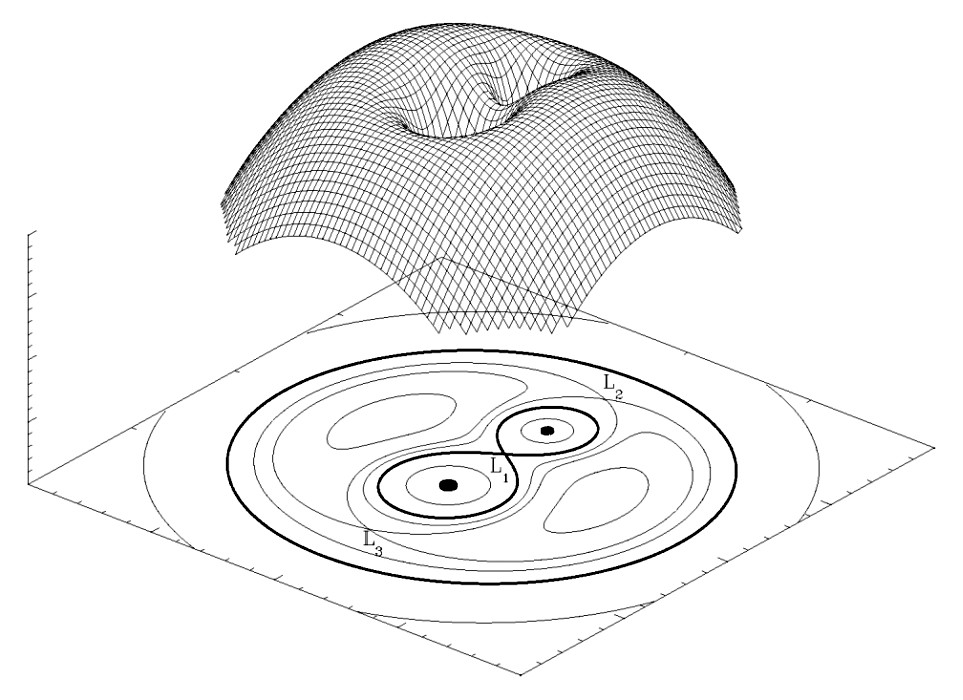
\includegraphics[width=\textwidth]{Figs/RochePotential.jpg}

        \subsection{\centering Detached}
        In systems which are regarded as detached, ie, neither star has filled its Roche Lobe mass transfer is still possible through a processed called Wind Accretion. We see this prominently in systems called \textit{High Mass X-ray Binaries}, where a supergiant star transfers mass to a compact object via wind accretion. This process leads to a increase in X-ray Emission, which we can measure.  \cite{TaurisvandenHeuvel+2023} It is important to note that these systems are not experiencing full-blown RLO, however, they tend to be incredibly close. \cite{TaurisvandenHeuvel+2023} This systems transfer mass through both wind accretion and in some cases, atmospheric RLO.

        I used the system Vela X-1 \cite{Kretschmar_2021} as a example of this, as it is generally regarded as the "archetypical wind accretor" \cite{Kretschmar_2021} 
        
        \begin{center}
            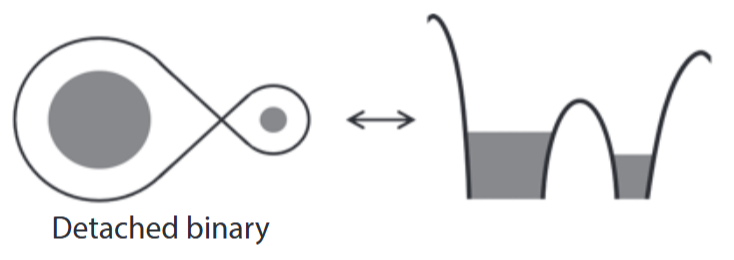
\includegraphics[scale = .4]{Figs/Detached binary.png}
        \end{center}
        
        \subsection{\centering Roche Lobe overflow} % maybe include equations??
        In systems where one star fills its gravitational potential mass begins to be transferred to its binary partner. This is called Roche Lobe Overflow (RLO) and is defined by a Donor and Accretor star. 

        We see this commonly in X-ray Binaries, where a donor star transferred mass to an accretor which is a compact object (either a neutron star (NS) or black hole (BH). This process then produces X-rays which we can measure to understand the processes within the binary in greater detail. This process is generally \textbf{\textit{directly}} in RLO through L$_1$. 
        
       \begin{center}
            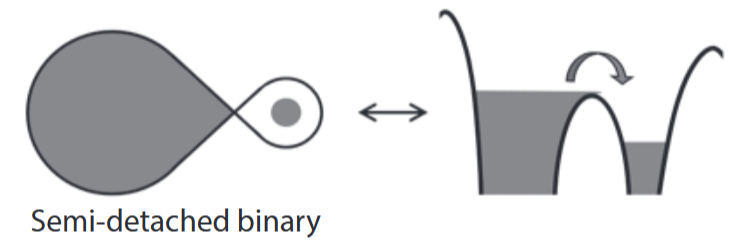
\includegraphics[scale = .4]{Figs/Semi-detached binary.png}
        \end{center}
        
        I used the system V404 cyngi with data from \cite{Bernardini_2016} and \cite{10.1093/mnras/271.1.L10} as as an example of this behavior. 
        
 
        

        \subsection{\centering Contact Binary}
        A Contact Binary occurs when both stars fill their potential and start filling up their systems potential, this leads to the sharing mass.
        
        \begin{center}
        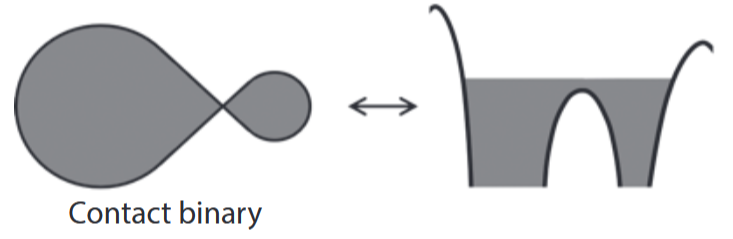
\includegraphics[scale = .4]{Figs/Conact Binary.png}
        \end{center}

        It is important to note that these contact binaries appear to be elongated towards each other. 

        Smth smth smth

        I used W Ursae Majoris (W UMa) as an example of these systems, as it is used an example system in order to categorize bthese contact binarys as a whole.

        % \subsection{\centering X-ray Binaries}
        % In binaries with compact objects accretors (BHs and WDs) we find a large amount of produced X-ray binaries. We see this as bright Xray sources in our skies (cite). These X-rays are produced through mass falling into the accretor, causing xrays. (cite)
        
\section{\centering Data Acquisition}
    \subsection{\centering Vela X-1 (Detached)}
    
        \subsubsection{Observed}
        \begin{center}
            \begin{tabular}{||c c c||} 
             \hline
             & Vela X-1 A & Vela X-1 B  \\ 
             \hline\hline
             Star Type & Neutron Star & Supergiant \cite{Kretschmar_2021} \\ 
             \hline
             Masses\(M_\odot\) & $\ge$ 1.8 \cite{Kretschmar_2021} & 20–30 \cite{Kretschmar_2021} \\
             \hline
             Radius & 11-12.5$_{KM}$ \cite{Kretschmar_2021} & 30 \(M_\odot\)
             \cite{Kretschmar_2021} \\ % note that the stars are not spherical
             \hline 
            \end{tabular}
        \end{center}
        Vela X-1 consists of a Neutron Star and Supergiant and is an Eclipsing and pulsing High Mass X-ray Binary (HMXB). This means that the Neutron star passed behind the Supergiant every 8.94 days \cite{Falanga_2015}, leading to a variable luminosity between $10^{36}$ $erg$ $s^{-1}$ and $10^{37}$ $erg$ $s^{-1}$. Additionally, the neutron star itself is spinning every 293 seconds. \cite{Kretschmar_2021}. 
        Vela X-1 is described as an archetypical wind accretor. This is because unlike some systems... (ie \cite{Kretschmar_2021}) 
            
            
        \subsubsection{Simulated}
        Simulated data is good because of xyz and is useful because of xyz. data was made using xyz

    \subsection{\centering W Ursae Majoris (Contact Binary)}
        \subsubsection{Observed}
        
        \begin{center}
            \begin{tabular}{||c c c||} 
             \hline
             & W UMa A & W UMa B \\ 
             \hline\hline
             Star Type & O-Type \cite{Antokhina_2011} & O-Type \cite{Antokhina_2011} \\ 
             \hline
             Masses\(M_\odot\) & 1.139 ± 0.019\cite{10.1093/mnras/staa3753} & 0.551 ± 0.006\cite{10.1093/mnras/staa3753} \\
             \hline
             Radius\(R_\odot\) & 1.092 ± 0.016\cite{10.1093/mnras/staa3753} & 0.792 ± 0.015\cite{10.1093/mnras/staa3753} \\
             \hline
             Temperature$K$ & 33750 \cite{Antokhina_2011}  & 33500 \cite{Antokhina_2011} \\
             \hline
             Luminosity\(L_\odot\) & 1.557 ± 0.166\cite{10.1093/mnras/staa3753} & 0.978 ± 0.071\cite{10.1093/mnras/staa3753}   \\ 
             \hline
            \end{tabular}
        \end{center}
        
        \subsubsection{Simulated}
        Simulated data is good because of xyz and is useful because of xyz. data was made using xyz

    \subsection{\centering Roche Lobe overflow in V404 Cyngi}
        \subsubsection{Observed}
        \begin{center}
            \begin{tabular}{||c c c||} 
             \hline
             & V404 Cyngi B (Donor) & V404 Cyngi A (Black Hole) \\ 
             \hline\hline
             Star Type & Early K-type Giant & Black Hole \\ 
             \hline
             Masses\(M_\odot\) & .7 \cite{Bernardini_2016} & 9 \cite{10.1093/mnras/271.1.L10} \\
             \hline
             Radius\(R_\odot\) & 6.0 \cite{10.1093/mnras/271.1.L10} &  \\
             \hline
             Temperature$K$ & 4800 \cite{10.1093/mnras/271.1.L10} & \\
             \hline
             Luminosity\(L_\odot\) & 10.2 \cite{10.1093/mnras/271.1.L10} &  \\ 
             \hline
        \end{tabular} 
        \end{center}
         Observed data of V404 Cyngi shows the mass of the black hole is 9\(M_\odot\). The Donar star properties 

        \subsubsection{Simulated}
        Simulated data is good because of xyz and is useful because of xyz. data was made using xyz

    \subsection{POSYDON Simulations}
         I used data generated by POSYDON \cite{Fragos_2023} in corroboration with three observed systems in order to fully understand the depth of the process of mass transfer in Binary Systems.
    \cite{TaurisvandenHeuvel+2023}


\section{\centering Results}
    Through my research I found these distinct types of evolutionary processes ... and their stages of evolution, causes and populations. 
    
        \subsection{\centering Detached}
        In detached binaries, there is still the possibility for mass transfer. These systems are typically called HMXBs. I found that these systems have a distribution as pictured. Note these systems are only ones with full blown RLO due to simulation of WA constraints
        \begin{center}
            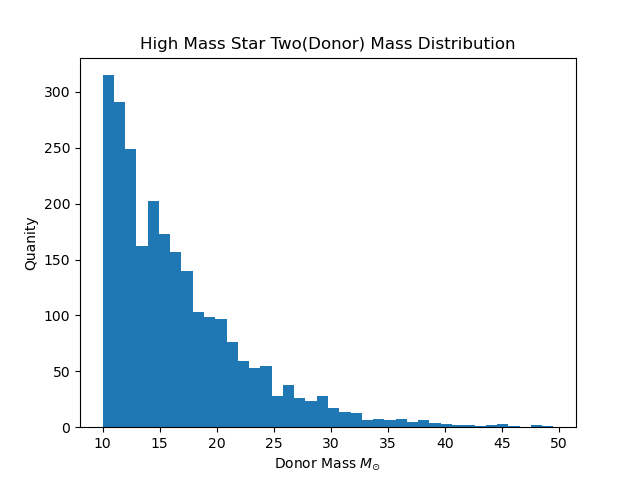
\includegraphics[scale = .6]{Figs/High Max X-ray Binary Star Two Mass Distro.png}
            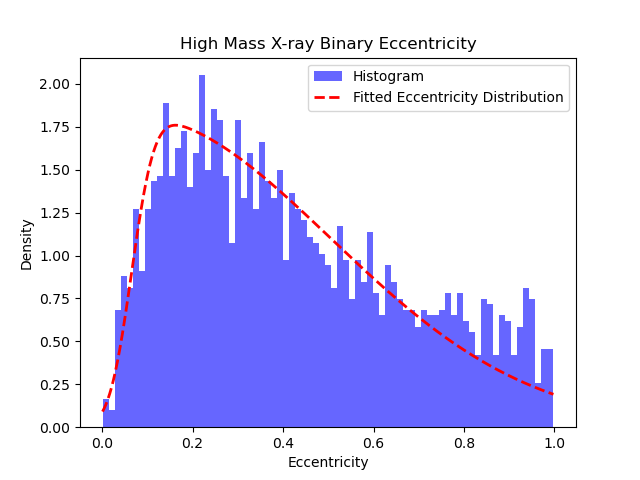
\includegraphics[scale =.6]{Figs/High Mass X-ray Binary Eccentricity.png}
        \end{center}
        Additionally, HMXBs fall in this region on the HR diagram 
        \begin{center}
            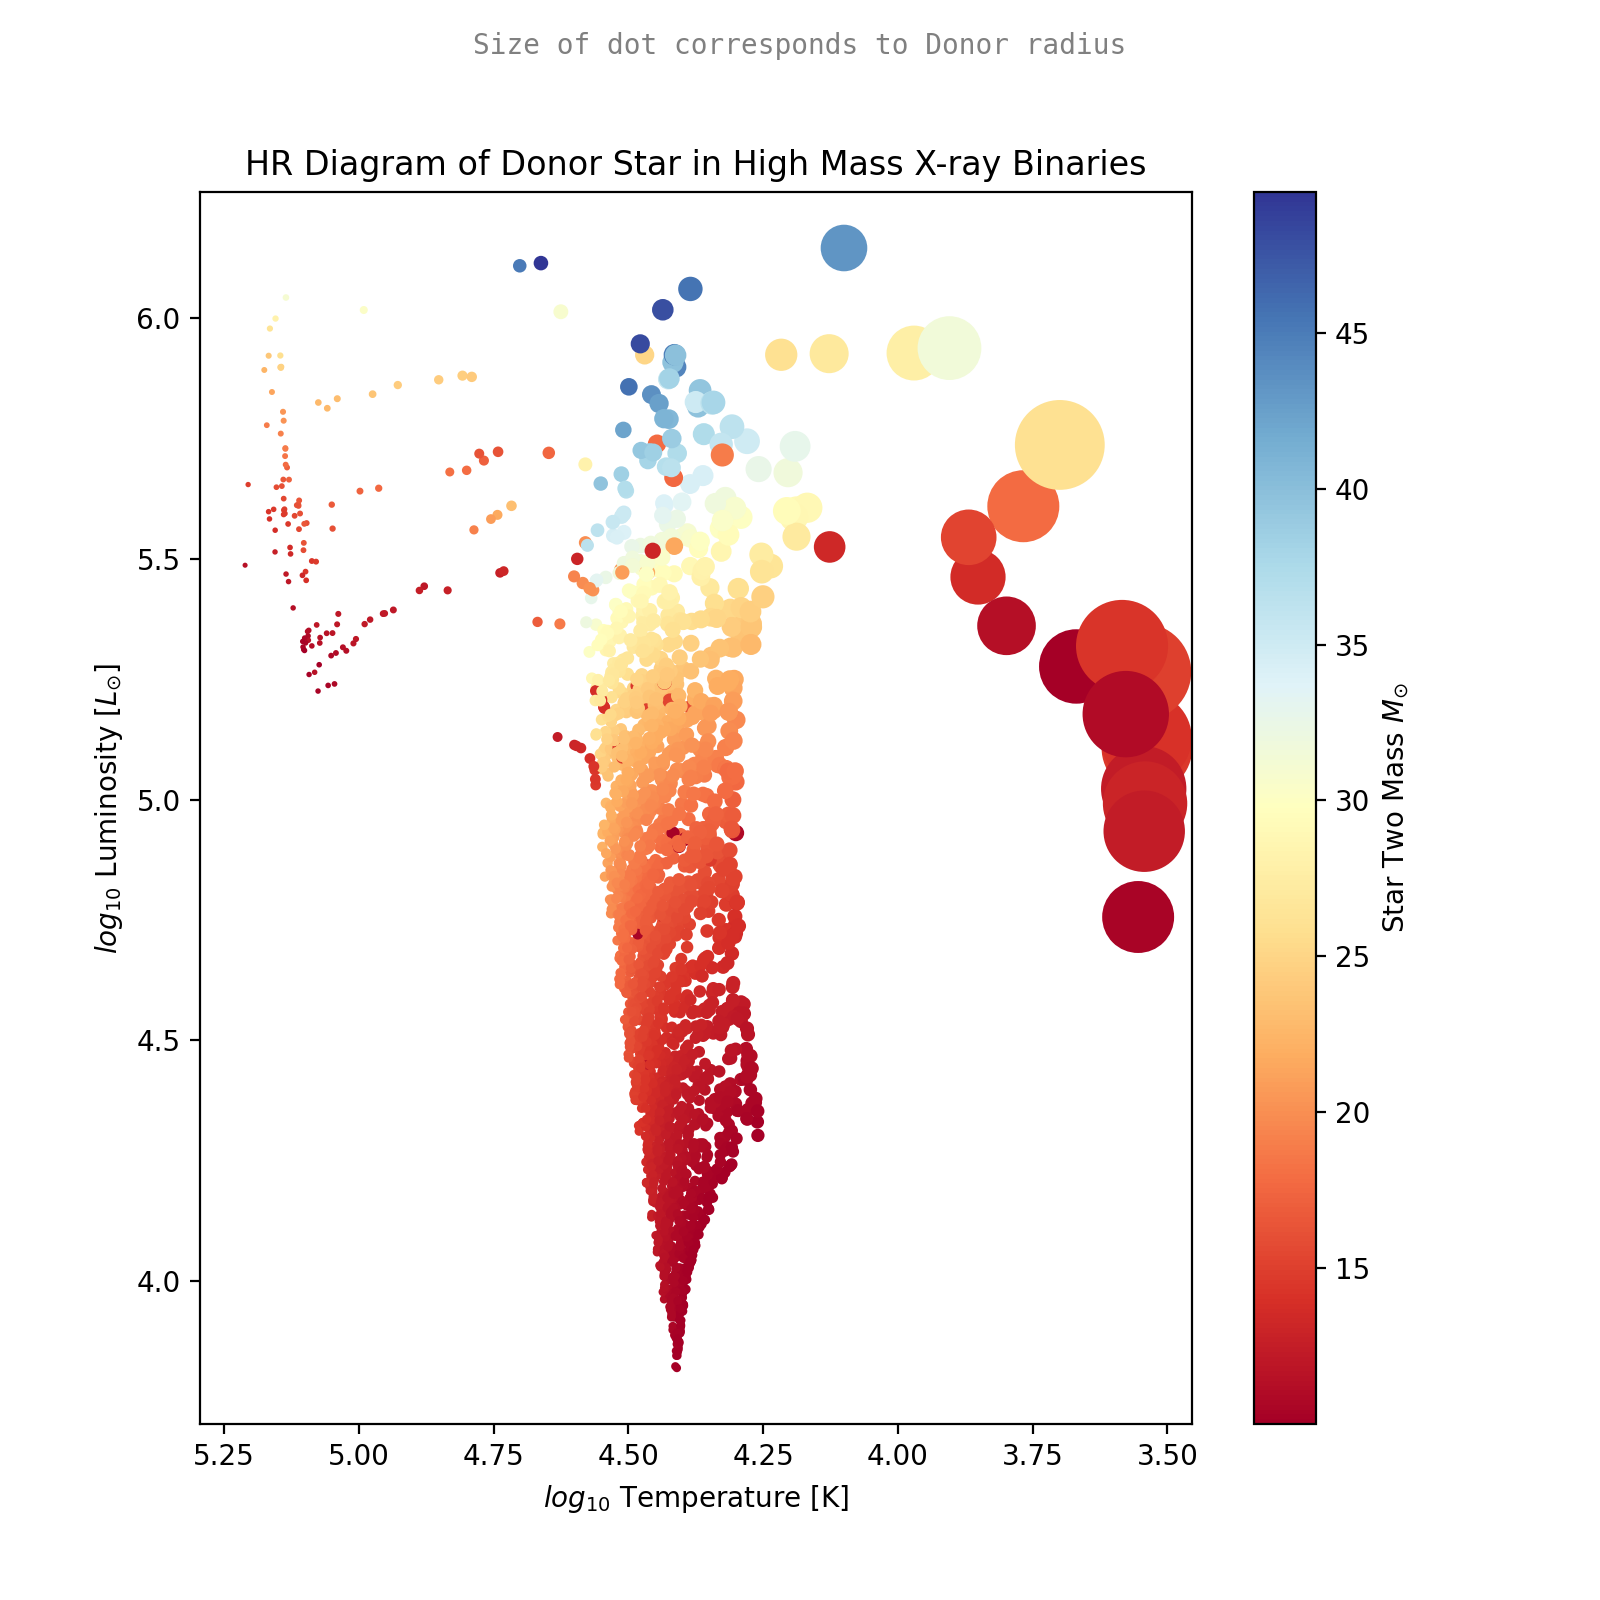
\includegraphics[scale = .5]{Figs/HR Diagram of Donor Star in High Mass Xray Binaries S2mass log10 F star radius T (2).png}
        \end{center}
  
        \subsection{\centering Roche Lobe Overflow}
        Full blown RLO occurs in both All of types of Xbs, including both HMXBs and LMXBs. This systems 
        \begin{center}
            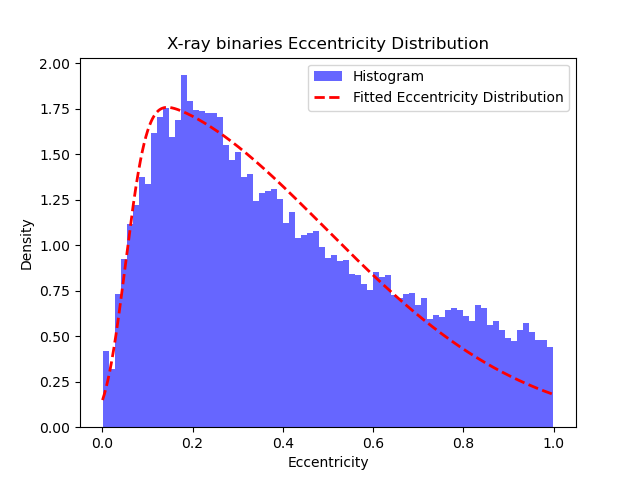
\includegraphics[scale=.5]{Figs/X-ray binaries Eccentricty Distribution.png}
            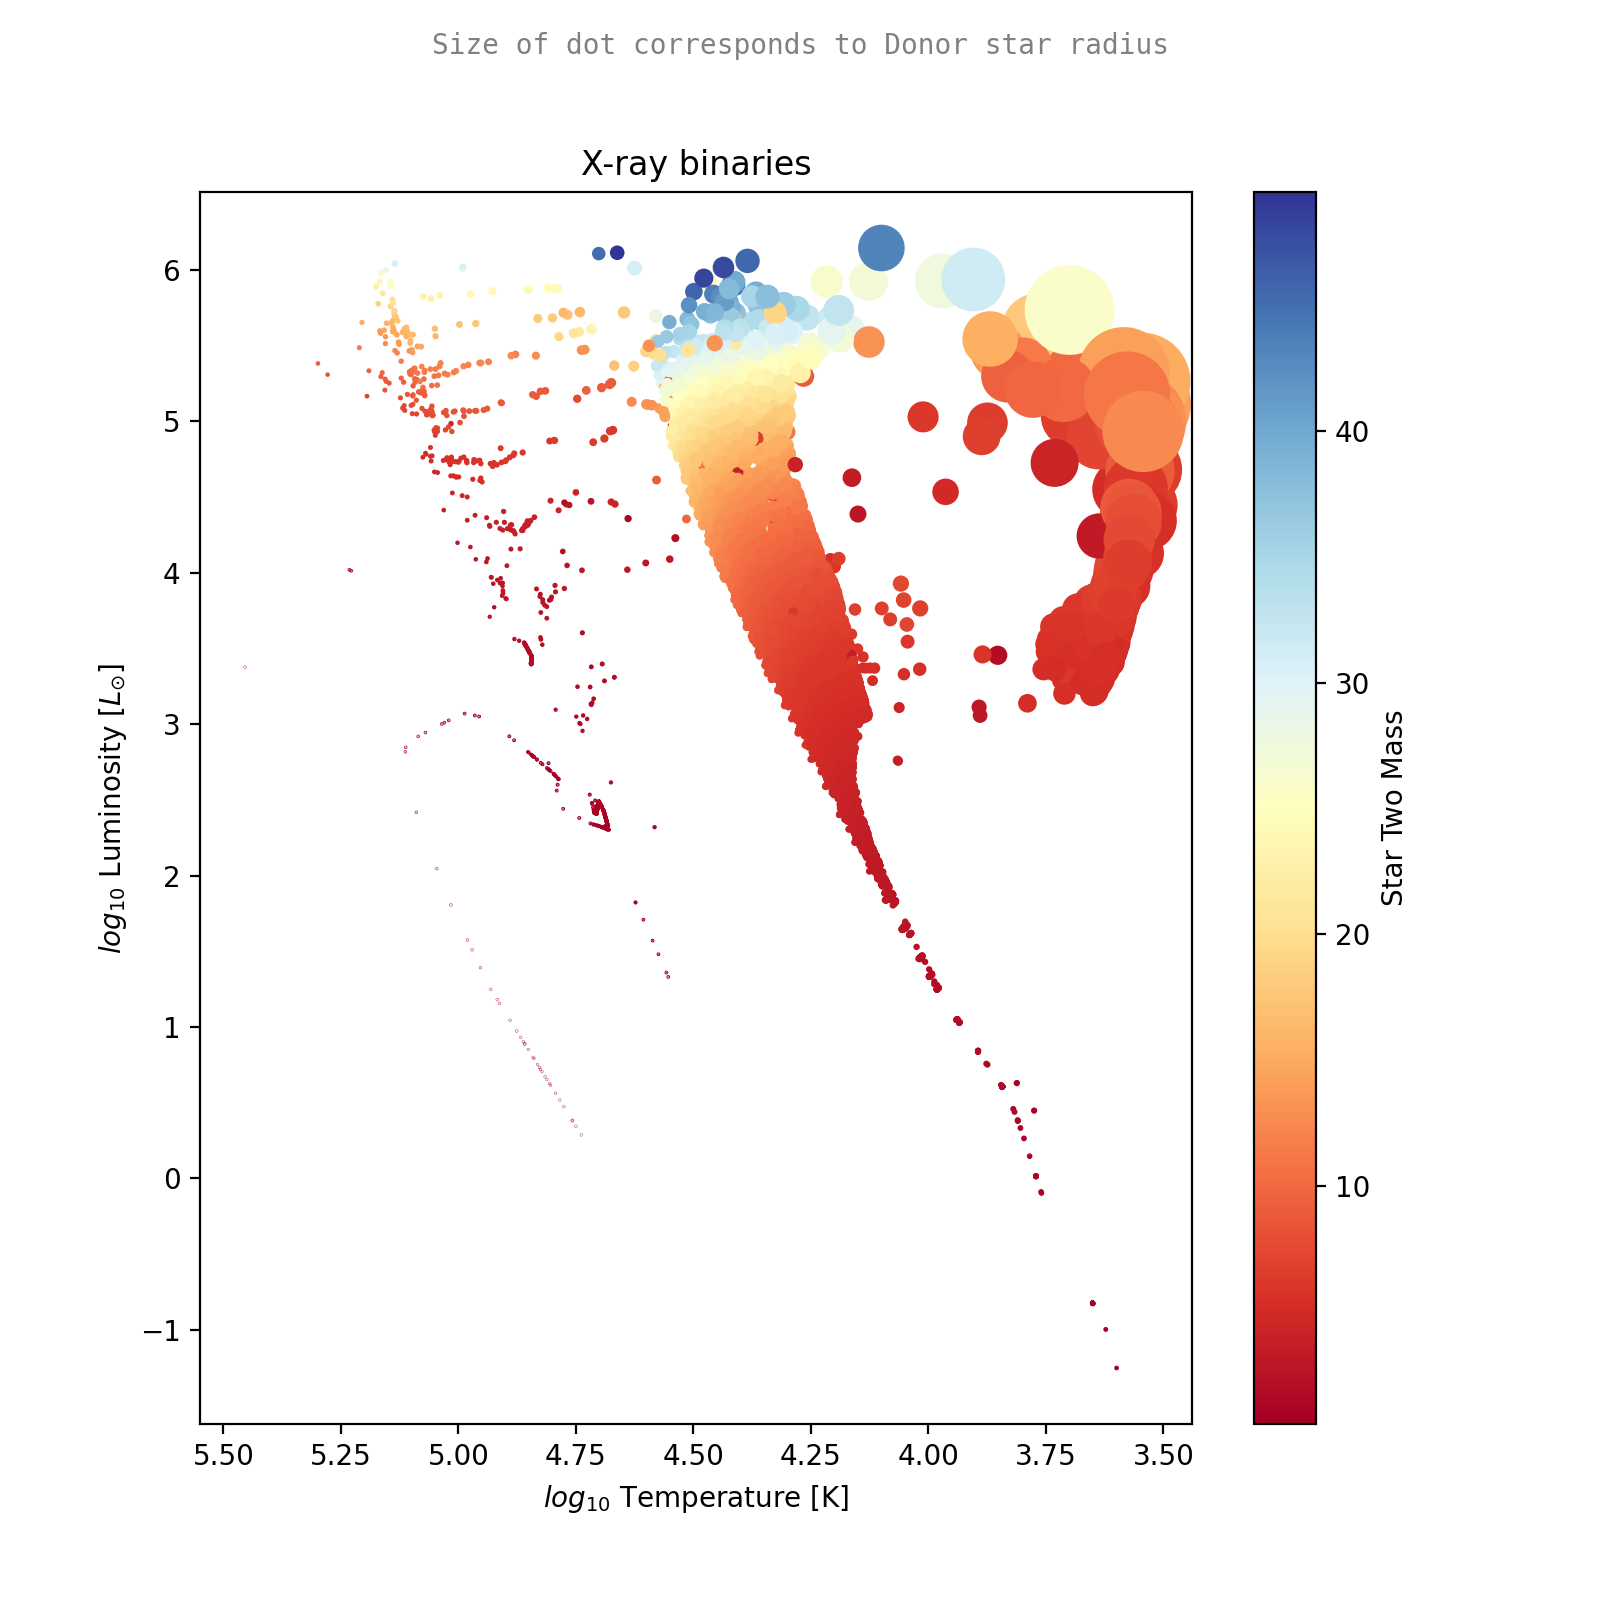
\includegraphics[scale=.5]{Figs/X-ray binaries S2mass log10 F star radius T.png}
            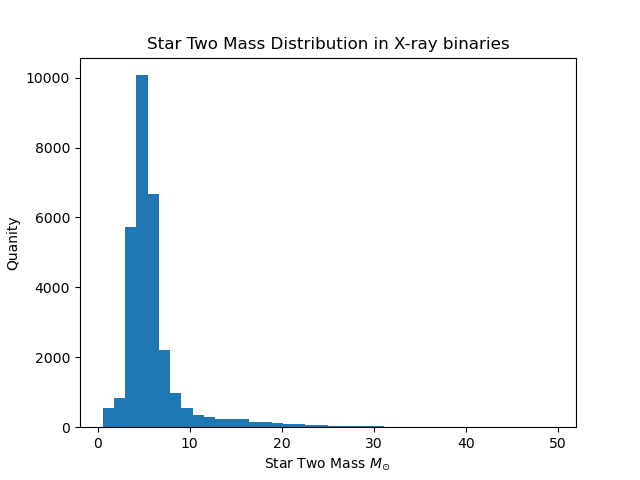
\includegraphics[scale=.6]{Figs/X-ray binaries Star Two Mass Distribution.png}
            
        \end{center}
        (cite and insert figs)
      
        \subsection{\centering Contact Binary}
        I found that in CE systems this can happen with these evolutionary changes. We see an example in observed systems (insert source and figs) in our POSYDON \cite{Fragos_2023} simulated data too. (figs)

        \begin{center}
            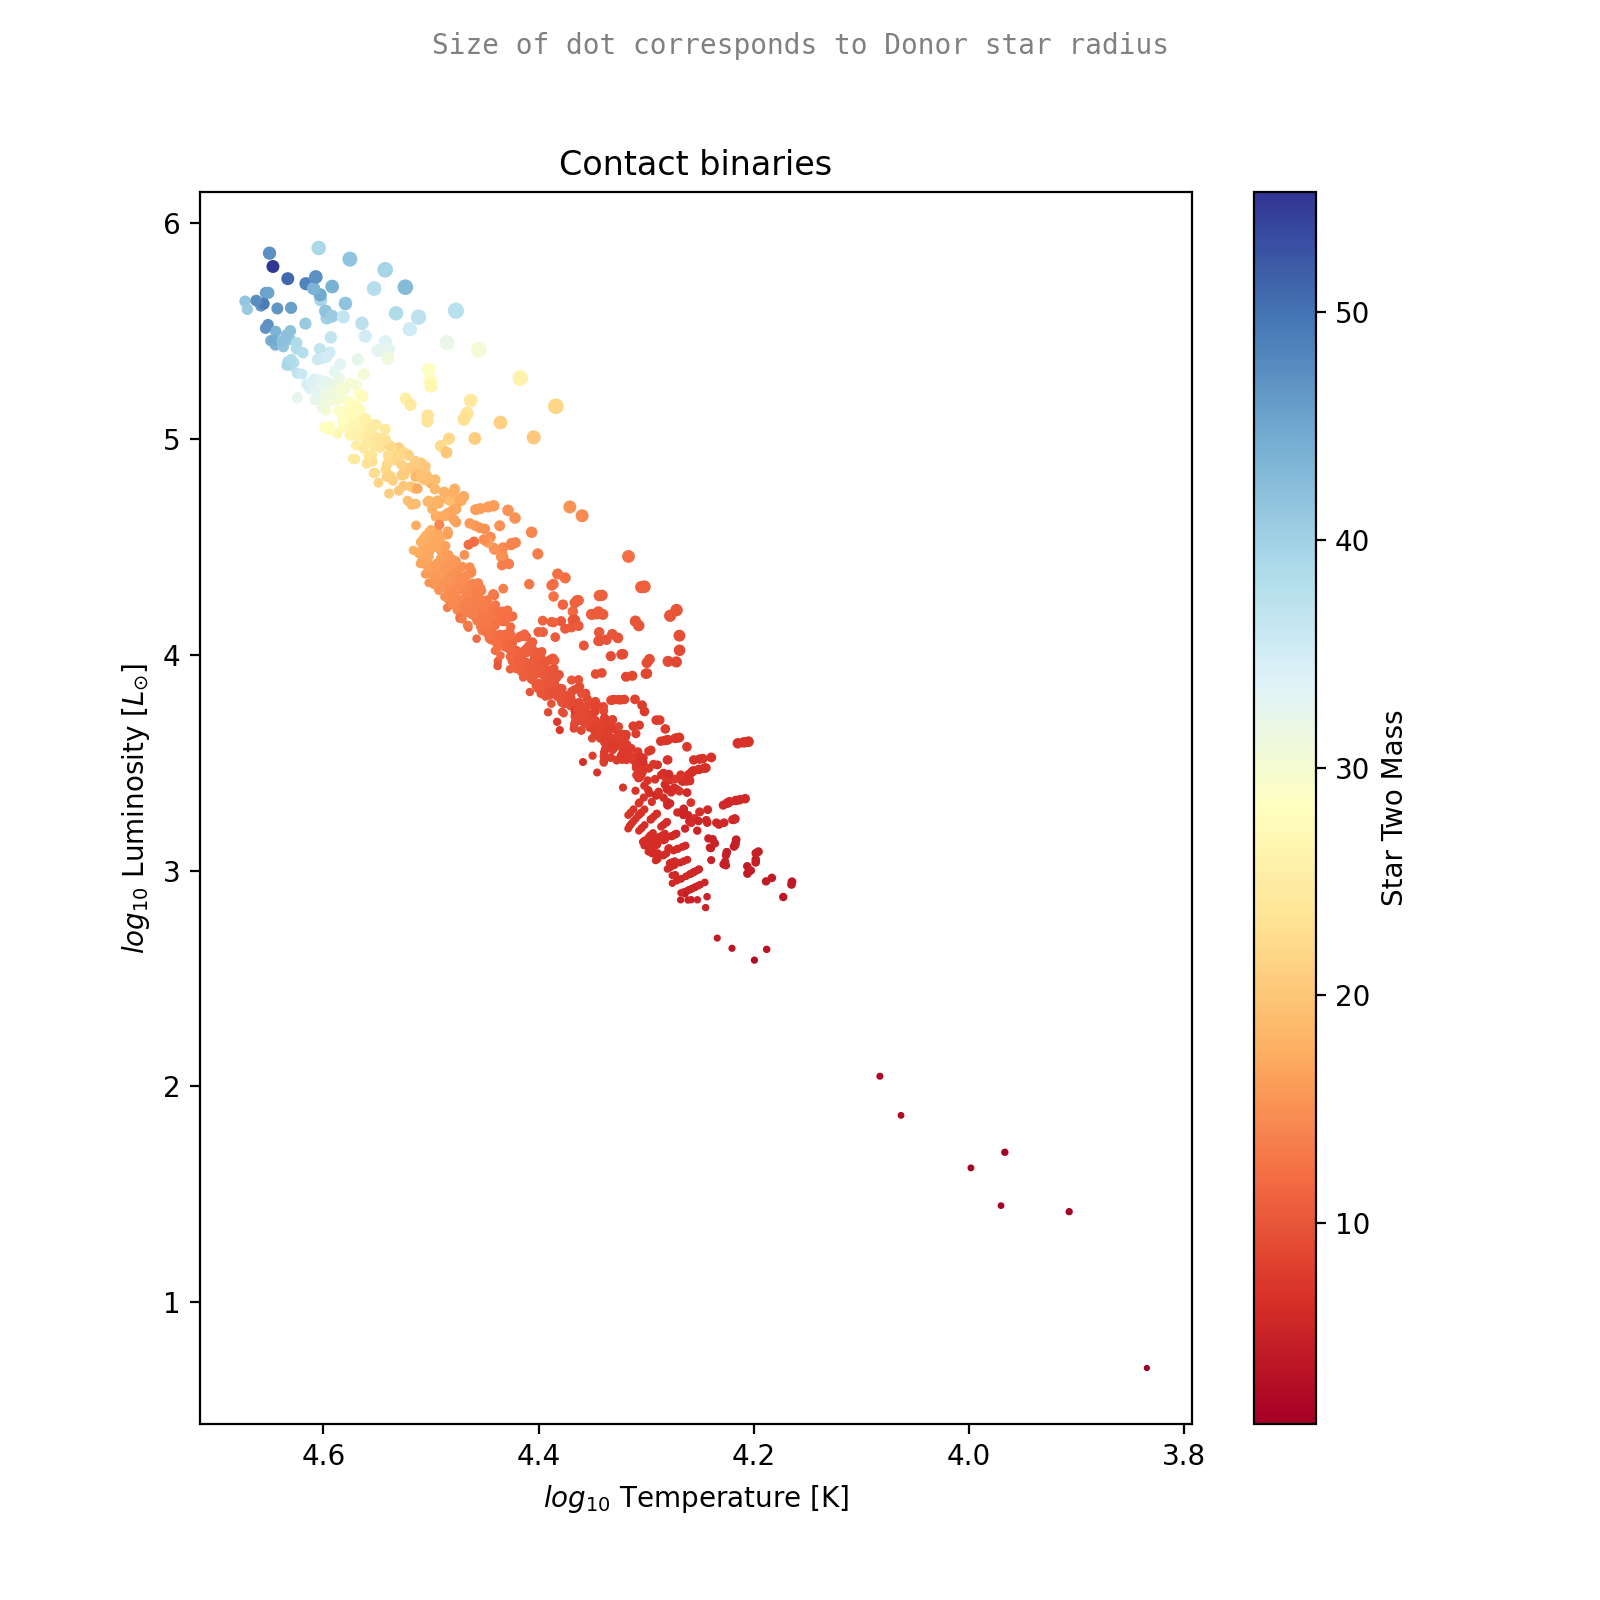
\includegraphics[scale = .6 ]{Figs/contact binary HR diagram.png}
            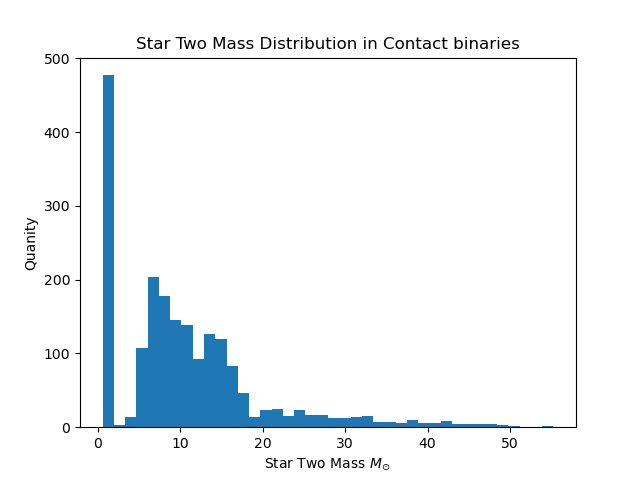
\includegraphics[scale = .5 ]{Figs/Contact binaries Star Two Mass Distribution.png}
        \end{center}
    % \subsection{\centering ii) Type 1a Supernova}
    % I found that in systems with type 1a SN the progenitors tend to be ..., this is corroborated with this paper (cite). We see a similarity with the POSYDON data and this papers data
 
    % \subsection{\centering iii) X-Ray Binaries}
    % I found that XrBs mass transfer effects them by causing changes to ... we see this our POSYDON data and this paper... 

\section{\centering Discussion}   
    originally I planned on simulating grids for all of the types of systems, however, due to time constraints I chose to only focus on one type. 
\section{\centering Conclusion}
    In conclusion mass transfer effects binary systems in these ways, which can lead to these evolutionary outcomes. 

\printbibliography[
heading=bibintoc,
title={\centering Sources}
]

\end{document}